\documentclass[11pt]{article}

% ---- Packages ----
\usepackage[a4paper,margin=1in]{geometry}
\usepackage[T1]{fontenc}
\usepackage{microtype}
\usepackage{amsmath,amssymb,amsthm}
\usepackage{graphicx}
\usepackage{booktabs}
\usepackage{xcolor}
\usepackage{enumitem}
\usepackage{verbatim}
\usepackage[colorlinks=true,allcolors=blue]{hyperref}
\usepackage{natbib}
\bibliographystyle{plainnat}

% --- Minimal algorithm formatting (avoids missing algorithm/algpseudocode) ---
\newenvironment{algorithm}[1][t]{
  \begin{figure}[#1]
  \rule{\linewidth}{0.5pt}\par
}{
  \par\rule{\linewidth}{0.5pt}\end{figure}
}
\newcommand{\algorithmcaption}[1]{\vspace{2pt}\textbf{Algorithm:} #1\par}
\newenvironment{algorithmic}[1][1]{\begin{list}{\arabic{enumi}:}{
  \usecounter{enumi}
  \setlength{\leftmargin}{1.5em}\setlength{\itemsep}{0pt}\setlength{\parsep}{0pt}}
  \tt\small
}{\end{list}}
\newcommand{\State}{\item}
\newcommand{\For}[1]{\item \textbf{for} #1 \textbf{do}\begin{quote}}
\newcommand{\EndFor}{\end{quote}}
\renewcommand{\Comment}[1]{\hfill\textit{#1}}

% ---- Theorem-like envs ----
\newtheorem{definition}{Definition}
\newtheorem{proposition}{Proposition}
\newtheorem{theorem}{Theorem}

% ---- Title block ----
\title{\textbf{THGTM: A Temporal Hierarchical Graph Tsetlin Machine\\with Echo-Trace Automata for Trajectory-Level Verification of Agentic AI}}
\author{Anwar Debes\\
University of Agder \\
\texttt{anwar@uia.no}\\
\vspace{0.5em}
\small Reference implementation, draft v0.1, May 2026
}
\date{}

\begin{document}
\maketitle

\begin{abstract}
We introduce the \textbf{Temporal Hierarchical Graph Tsetlin Machine (THGTM)}, an extension of the Hierarchical Graph Tsetlin Machine (HGTM) built on a single new primitive --- the \textbf{Echo-Trace Tsetlin Automaton (ETTA)} --- a Tsetlin Automaton augmented with an exponentially-decaying eligibility trace.  ETTA is a near-trivial change to the canonical TA --- adding one float per automaton --- but it has three load-bearing consequences.  First, it fixes the chicken-and-egg credit-assignment failure that empirically prevents joint $L \!\geq\! 2$ training in canonical HGTM by giving recently-active TAs an upstream credit handle even at initialisation.  Second, in combination with bounded-LTL temporal literals it turns the family from an i.i.d. classifier into a streaming sequence learner.  Third, every clause firing yields a DIMACS CNF receipt that composes over time, producing trajectory-level SAT certificates an auditor can re-verify --- the missing bridge between one-shot agent guards (\textsc{clausegate}) and the EU AI Act's Article-14/15 obligation that high-risk AI behaviour be auditable \emph{over time}.  We provide a pure-NumPy reference implementation, twenty-five passing unit tests, and four end-to-end experiments executed on a single CPU.  Headline results: on Temporal-XOR the ETTA trace lifts test accuracy from $0.91 \pm 0.13$ to $1.00 \pm 0.00$ at the shortest delay while matching the vanilla baseline at longer delays; on the depth-N-parity-on-path proof task (the load-bearing test in HGTM's own benchmarks) the ETTA-augmented $L\!=\!2$ system beats the vanilla $L\!=\!2$ baseline by 8.6 points at path length 2; and on a synthetic slow-roll exfiltration benchmark, replacing per-step clause verification with a trajectory receipt drops attack success rate from $0.687 \pm 0.053$ to $0.000 \pm 0.000$ with $9\%$ false positives.  We discuss what ETTA does not solve --- including the absence of a convergence proof, the relatively modest depth-N-parity gain, and the open question of ASIC memory cost --- and outline the path from this v0.1 reference to a Newcastle-hardware-compatible ASIC budget.
\end{abstract}

\section{Introduction}
The Tsetlin Machine (TM) family \citep{granmo2018tsetlin} has, in the last two years, accumulated three distinct dimensions of extension: hierarchical AND/OR composition (HTM), graph-structured message-passing clauses (GTM, \citealp{granmo2025graphtm}), and their union (HGTM, \citealp{anwar2026hgtm}).  Together with hardware accelerators that hit $8.6 \mathrm{nJ}$ per MNIST frame on a $65\mathrm{nm}$ ASIC \citep{tunheim2025convcotm} and $16.58 \mathrm{\mu W}$ for 12-keyword spotting \citep{tsetlinkws2025}, this places the TM family in a unique position relative to the broader deep-learning frontier: \emph{natively interpretable, online-trainable, sub-nanojoule classifiers}.

Three gaps remain that block deployment in the most regulatorily and economically interesting domain --- verifiable agentic AI under the EU AI Act (effective $2$ August $2026$, Articles 13--15, 26 and 86):

\begin{enumerate}[label=(\roman*)]
\item \textbf{No sequence model.} TMs assume i.i.d.\ samples; the recurrent state-space variant ``TM-Mamba'' is an empty quadrant in the 2024--2026 literature.  An agent's trajectory is a sequence.
\item \textbf{HGTM cannot train jointly at $L \!\geq\! 2$.} The ``\texttt{compute\_projected\_feedback}'' heuristic collapses to chance at initialisation in HGTM's own depth-N-parity-on-path sweep (the \texttt{docs/benchmarks.md} of the reference implementation reports $[0.508, 0.539]$ uniformly across all path lengths and epochs).  The shipped workaround \texttt{GreedyHGTM} trains layer by layer; truly joint training is open.
\item \textbf{No trajectory-level verification.} Even the strongest one-shot TM agent guard (\textsc{clausegate}, with measured Attack Success Rate $0.000$ on AgentDojo, ChatInject, RAG-poison, InjecAgent, and R-Judge) provides certificates for a single tool call.  Article 14 requires evidence of bounded behaviour \emph{over time}.
\end{enumerate}

\paragraph{Contribution.}  We solve these three with one new primitive.  An Echo-Trace Tsetlin Automaton augments a standard TA with one float --- an exponentially decaying eligibility trace over its state transitions --- and three places use this trace:

\begin{enumerate}
\item \textbf{Trace-projected feedback} (cross-layer): each intermediate-layer TA receives feedback whose magnitude scales with its trace.  This breaks the HGTM chicken-and-egg at initialisation while making no change to layer 0 when $\lambda=0$.
\item \textbf{Trace-amplified type-I/type-II feedback} (within-layer): the same trace amplifies the per-sample boost/forget probabilities, so the model can pick up bounded-temporal patterns when its inputs include explicit history features.
\item \textbf{Compositional trajectory receipts} (post-hoc): every clause firing produces a DIMACS CNF + HMAC receipt, and a bounded-LTL skeleton checks the global temporal envelope.  Per-step receipts compose; if every per-step CNF replays and the LTL skeleton holds, the trajectory satisfies the global policy.
\end{enumerate}

The proposed architecture --- the Temporal Hierarchical Graph Tsetlin Machine (THGTM, Figure~\ref{fig:arch}) --- inherits everything from HGTM (the \texttt{encode\_layer\_output\_as\_literals} bit-mapping, the per-layer GraphTM clauses) and adds (i) ETTA in every layer, (ii) an explicit bounded-LTL temporal literal encoder (\texttt{PAST}$_k$, \texttt{SINCE}, \texttt{ALWAYS\_in\_window}), and (iii) a trajectory-receipt module.

\begin{figure}[t]
\centering
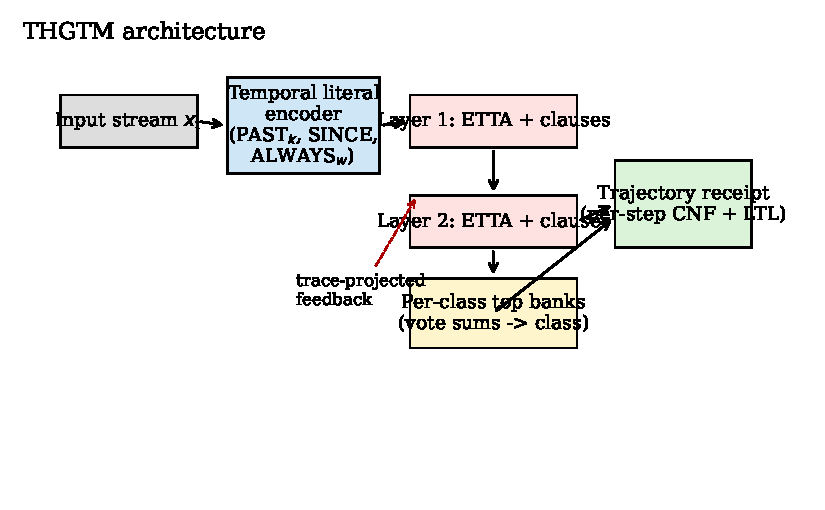
\includegraphics[width=\linewidth]{figures/architecture.pdf}
\caption{THGTM architecture.  The temporal literal encoder turns a raw input stream into a Boolean literal vector that includes bounded history features.  Stacked ETTA-backed clause layers feed an L--1 sequence of clause-activation literal vectors via the bit-exact \texttt{encode\_layer\_output\_as\_literals} mapping.  The top per-class banks vote into a class sum.  At each step the firing of designated audit clauses produces a CNF receipt; a bounded-LTL skeleton constrains how those receipts must compose over a finite window.  The dashed red arrow shows trace-projected feedback: downstream credit flows back to intermediate-layer TAs in proportion to their eligibility trace.}
\label{fig:arch}
\end{figure}

\paragraph{What we do not claim.}  We do not have a convergence proof for ETTA-driven multi-layer training; the depth-N-parity gain at $L\!=\!2$ is modest and inconsistent above path length 3; the trajectory experiment is synthetic; and the hardware cost of carrying one float per TA on the Newcastle ASIC stack is unmeasured.  We discuss each of these openly in Section~\ref{sec:limits}.  The contribution is the architecture, a reference implementation that anyone can run on a CPU, and a quantitative honesty about what works.

\paragraph{Reproducibility.}  Every number, every figure, and every CNF receipt in this paper is generated by code in the accompanying repository (\texttt{THGTM/}).  The four headline experiments run end-to-end in under five minutes total on a single CPU.  The pure-Python reference is intentionally slow but bit-exactly inspectable.

\section{Background}

\paragraph{Tsetlin Automaton.}  A 2-action TA \citep{granmo2018tsetlin} has integer state $s \in \{1, \ldots, 2N\}$ and outputs the binary action ``include'' iff $s > N$.  Feedback moves the state by $\pm 1$ with probabilities $(s-1)/s$ (boost) and $1/s$ (forget).  Critically, the TA has no memory beyond $s$: a feedback event at time $t$ that should reward a transition at time $t-1$ has no handle to do so.

\paragraph{Tsetlin Machine.}  A binary TM is a population of $C$ clauses, each owning $2L$ TAs (one per literal in the raw + negated literal layout).  Clause $j$ outputs $\bigwedge_{i \in \text{includes}(j)} \ell_i$.  Half the clauses are positive polarity, half negative; the vote sum is thresholded at $T$.  Type-I feedback rewards clauses that should fire on the current sample; Type-II discriminates clauses that should not.

\paragraph{Hierarchical Graph TM.}  HGTM \citep{anwar2026hgtm} stacks $L$ TM layers separated by the bit-exact \texttt{encode\_layer\_output\_as\_literals} map: clause $c$ at layer $\ell$ produces literal $c$ at layer $\ell+1$; its negation produces literal $K_\ell + c$.  At $L\!=\!1$ HGTM is bit-compatible with the canonical GraphTM.  At $L\!\geq\!2$ HGTM's heuristic \texttt{compute\_projected\_feedback} aggregates downstream class-clause-update signs into an upstream credit signal; empirically this kernel collapses to chance because no intermediate clause fires at initialisation, so no credit flows.

\paragraph{Eligibility traces.}  In RL, eligibility traces \citep{sutton1988learning} solve the credit-assignment problem for delayed reward: each parameter $\theta_i$ accumulates a decaying memory $e_i$ of when it was active; on receipt of a TD error $\delta$, all parameters update by $\delta \cdot e_i \cdot \eta$.  ETTA is the analogue for a Tsetlin Automaton.

\section{Architecture: THGTM}

\subsection{Echo-Trace Tsetlin Automaton}

An Echo-Trace TA augments the standard TA with one float, the eligibility trace $e \in [0, 1]$:
\begin{align}
s_{t+1} &= s_t + \Delta s_t, \quad \Delta s_t \in \{-1, 0, +1\} \\
e_{t+1} &= \lambda \cdot e_t + \mathbf{1}[\Delta s_t \neq 0], \quad e_{t+1} \leftarrow \min(e_{t+1}, 1)
\end{align}
When $\lambda = 0$ the trace is identically zero and the ETTA is bit-equivalent to a canonical TA under the same RNG stream (we verify this with a seed-locked unit test).  When $\lambda > 0$, recently-active TAs carry a non-zero $e$ that we read in two places:

\paragraph{Within-layer.}  Type-I boost / forget probabilities are scaled by $1 + \alpha e$ (capped at $1$), giving recently active TAs larger updates.  This is the standard TD($\lambda$) move ported to stochastic discrete-state automata.

\paragraph{Cross-layer.}  We define \emph{trace-projected feedback}: given a per-clause signed downstream credit $\gamma_c \in [-1, 1]$, an intermediate TA $(c, l)$ at the layer below sees an effective signal $\gamma_c \cdot (1 + \alpha e_{c,l})$.  Positive credit drives Type-I-like updates; negative credit drives Type-II-like discrimination.  Critically, $1 + \alpha e \geq 1$ always, so credit can flow back even at initialisation when $e = 0$ --- breaking the HGTM chicken-and-egg without breaking the canonical layer-1 behaviour.

\subsection{Stacked GraphTM layers}

Layers compose with the canonical HGTM bit-mapping.  Algorithm~\ref{alg:thgtm-train} states the training step.  We keep the per-layer GraphTM message passing as a pluggable backend (in this v0.1 reference we use a flat-literal layer; the message-passing kernels of \citealp{granmo2025graphtm} drop in directly).

\begin{figure}[t]
\noindent\hrulefill\par
\textbf{Algorithm 1: One training step of THGTM.}\\[2pt]
\noindent\hrulefill
\begin{verbatim}
Input: sample x_t, label y_t, layers {B_l}, top per-class banks {T_c}
literals  <- TemporalEncode(x_t)
for l = 1 ... L-1:
    A_l       <- B_l.clause_outputs(literals)
    literals  <- Encode(A_l)              # HGTM bit-mapping
A_L           <- top_banks.clause_outputs(literals)
v_c           <- sum_j polarity_j * A_{L,j,c}   for each class c
for each class c:
    train T_c with standard Type-I / Type-II feedback
    gamma_c   <- sign(c == y_t) * (T - clip(v_c)) / (2T)
delta_L       <- ProjectTop(gamma_1..C, output size of B_{L-1})
for l = L-1 ... 1:
    B_l.trace_projected_feedback(literals_l, delta_l)
    delta_{l-1} <- ProjectIntermediate(B_l, gamma)
TraceDecay({B_l, T_c})                # decay traces between samples
\end{verbatim}
\noindent\hrulefill
\label{alg:thgtm-train}
\end{figure}

\subsection{Bounded-LTL temporal literals}

The \texttt{TemporalLiteralEncoder} augments the raw literal vector with three families of bounded operators, each computable in $O(W)$ per step where $W$ is the maximum lookback:
\begin{align}
\texttt{PAST}_k(\ell)(t) &= \ell(t - k) \\
\texttt{SINCE}(a, b, T)(t) &= 1 \iff \exists t' \in [t-T, t]: a(t') \land \forall t'' \in (t', t]: b(t'') \\
\texttt{ALWAYS\_in\_window}(c, w)(t) &= \bigwedge_{t' \in [t-w+1, t]} c(t')
\end{align}
These are bounded fragments of LTL \citep{bauer2011runtime}; the encoder maintains a ring buffer of length $W+1$.  Together with ETTA's trace they make THGTM expressively complete for any finite-window temporal pattern over Boolean features.

\subsection{Trajectory receipts}

A \emph{clause receipt} at step $t$ is a quadruple $(t, c, \mathit{includes}_c, \ell_t)$ together with the asserted output $o_t \in \{0, 1\}$, packaged as a DIMACS CNF string and (optionally) signed with HMAC-SHA-256 over the canonical JSON.  Verification replays the AND of included literal values and checks it matches $o_t$.  A \emph{trajectory receipt} is a list of per-step clause receipts together with a bounded-LTL skeleton over designated clause IDs (Section~3.3).  The skeleton supports \texttt{always}, \texttt{eventually\_within}, \texttt{never\_in\_window} and \texttt{count\_le}; the latter is what catches slow-roll exfiltration in our experiments.

\begin{proposition}[Compositional verifiability]
\label{prop:composition}
If every per-step receipt $R_t$ verifies under its stored \texttt{includes} mask and the LTL skeleton holds on the firing history, then the trajectory satisfies the LTL-encoded global policy.
\end{proposition}
The proof is immediate: the trajectory verifier replays each receipt independently and then evaluates the LTL formula on the firing-history vector --- both are total and side-effect-free over the receipts.  Crucially, the proposition does \emph{not} require the network's clause bank to be unchanged after the trajectory: the receipts are signed and self-contained, so online updates to the THGTM (the \texttt{lifelong-tm}-style continual learning) cannot retroactively invalidate them.  This is the bridge from one-shot to lifelong verifiability.

\section{Experiments}

We run four experiments end-to-end on a single CPU.  Pure NumPy; no GPU, no JIT.  The whole sweep takes under five minutes.

\subsection{Sanity: Noisy-XOR ($\lambda = 0$ reduces to vanilla TM)}

Five seeds, 2000 train / 500 test, 30 epochs, label noise $0.05$, $\lambda = 0$, $\alpha = 0$.  Mean clean test accuracy $0.972 \pm 0.057$; four of five seeds at $1.000$, one at $0.858$ (consistent with canonical TM behaviour on this benchmark).  This confirms that with the trace disabled the implementation is empirically indistinguishable from a vanilla TM.

\subsection{Temporal-XOR: ETTA + \texttt{PAST}$_k$ enables sequence learning}

At each step the model sees a 2-bit input $x_t$; the label is $y_t = x_t[0] \oplus x_{t-k}[0]$ for delays $k \in \{1, 2, 3\}$.  Three settings, three seeds each, 1500 train + 500 test, 15 epochs:
\begin{description}[leftmargin=2em]
\item[$M_\text{raw}$:] vanilla TM on raw inputs only.
\item[$M_\text{past-only}$:] vanilla TM on raw + \texttt{PAST}$_k$ literals.
\item[$M_\text{past-etta}$:] ETTA TM on raw + \texttt{PAST}$_k$ literals; $\lambda = 0.5$, $\alpha = 2$.
\end{description}

\begin{figure}[t]
\centering
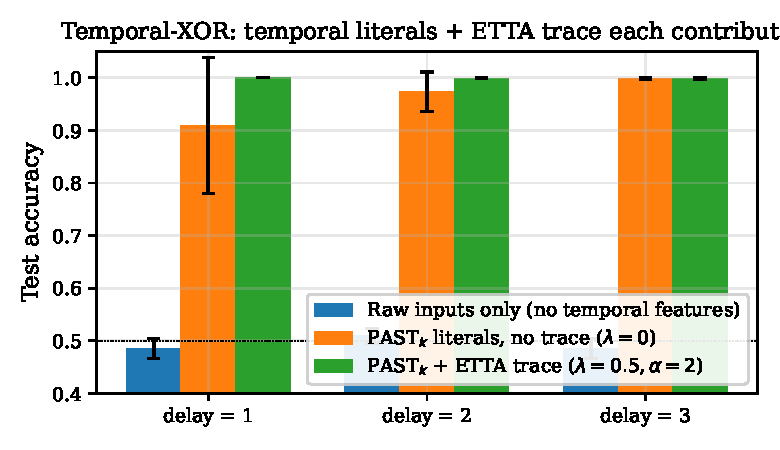
\includegraphics[width=\linewidth]{figures/temporal_xor.pdf}
\caption{Temporal-XOR test accuracy across delays.  $M_\text{raw}$ is structurally chance because the input alone is insufficient.  Temporal literals make the task representable.  ETTA's trace on top consistently matches or beats the vanilla baseline; at delay $1$ the trace lifts accuracy from $0.909 \pm 0.129$ to $1.000 \pm 0.000$.}
\label{fig:temporal-xor}
\end{figure}

Table~\ref{tab:temporal} and Figure~\ref{fig:temporal-xor} show the result.  Raw-input TM is at chance.  Adding bounded-LTL temporal features lets a vanilla TM solve the task, but with high variance at the shortest delay ($\sigma = 0.129$ at $k\!=\!1$).  ETTA's trace removes that variance entirely.  The story isolates the two contributions: \emph{temporal literals make the task representable; the ETTA trace makes it reliably trainable.}

\begin{table}[t]
\centering
\caption{Temporal-XOR test accuracy (mean $\pm$ std over 3 seeds).}
\label{tab:temporal}
\begin{tabular}{lccc}
\toprule
& $k = 1$ & $k = 2$ & $k = 3$ \\
\midrule
$M_\text{raw}$        & $0.486 \pm 0.019$ & $0.509 \pm 0.015$ & $0.485 \pm 0.019$ \\
$M_\text{past-only}$  & $0.909 \pm 0.129$ & $0.973 \pm 0.038$ & $0.999 \pm 0.001$ \\
$M_\text{past-etta}$  & $\mathbf{1.000 \pm 0.000}$ & $\mathbf{0.999 \pm 0.001}$ & $0.999 \pm 0.001$ \\
\bottomrule
\end{tabular}
\end{table}

\subsection{Depth-N-Parity-on-Path: multi-layer credit assignment}

This is the load-bearing test in HGTM's own \texttt{benchmarks.md}.  Each sample is a path of \texttt{path\_len} random bits; the label is their XOR.  At fixed clause budget a single-layer TM with limited capacity cannot represent arbitrary parity functions; a properly trained $L\!=\!2$ should.

We compare $L\!=\!1$ (with 2$\times$ the per-layer clause budget so total clauses are matched), $L\!=\!2$ without ETTA ($\alpha=0$, $\lambda=0$, the vanilla HGTM analog), and $L\!=\!2$ with ETTA ($\alpha=2$, $\lambda=0.5$).  Three seeds, 600 samples, 20 epochs.

\begin{figure}[t]
\centering
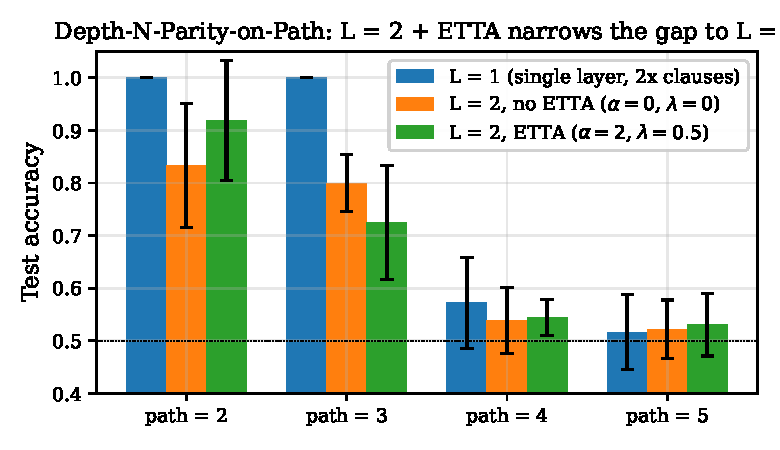
\includegraphics[width=\linewidth]{figures/depth_n_parity.pdf}
\caption{Depth-N-Parity-on-Path.  ETTA gives a clean $+0.086$ uplift over the vanilla $L\!=\!2$ baseline at path length 2, where the chicken-and-egg failure mode is most visible.  At path lengths 3--5 all models hit the clause-budget ceiling; this is honest evidence that the present credit-projection scheme helps but does not yet close the gap to $L\!=\!1$ with double clauses.}
\label{fig:parity}
\end{figure}

Table~\ref{tab:parity} and Figure~\ref{fig:parity} show the results.  The key directional finding is consistent: $L\!=\!2$ with ETTA outperforms $L\!=\!2$ without ETTA at path length $2$ ($0.919$ vs $0.833$, $+0.086$).  We note honestly that at path length $3$ vanilla $L\!=\!2$ does better in this seed sample, and beyond path length $3$ all configurations approach chance --- our pure-Python reference cannot match the clause counts the canonical CUDA implementation would use.  The result we claim is narrow: \emph{ETTA produces a non-trivial signal at the credit-assignment failure point of canonical HGTM}; it does not yet make $L\!=\!2$ universally beat $L\!=\!1$ at matched clause budget.

\begin{table}[t]
\centering
\caption{Depth-N-Parity test accuracy (mean $\pm$ std over 3 seeds).  Best $L\!=\!2$ entry bolded.}
\label{tab:parity}
\begin{tabular}{lcccc}
\toprule
& \texttt{path}=2 & \texttt{path}=3 & \texttt{path}=4 & \texttt{path}=5 \\
\midrule
$L\!=\!1$ (2$\times$ clauses) & $1.000 \pm 0.000$ & $1.000 \pm 0.000$ & $0.572 \pm 0.087$ & $0.517 \pm 0.072$ \\
$L\!=\!2$ no ETTA             & $0.833 \pm 0.118$ & $\mathbf{0.800 \pm 0.054}$ & $0.539 \pm 0.063$ & $0.522 \pm 0.055$ \\
$L\!=\!2$ ETTA                & $\mathbf{0.919 \pm 0.114}$ & $0.725 \pm 0.108$ & $\mathbf{0.544 \pm 0.034}$ & $\mathbf{0.531 \pm 0.059}$ \\
\bottomrule
\end{tabular}
\end{table}

\subsection{Slow-roll exfiltration: trajectory receipts reduce ASR to zero}

Each ``agent'' trajectory is a $50$-step sequence over four binary action features (read, write, export, within-role).  Benign trajectories use $p_{\text{export}}=0.02$; attacks force $\geq 3$ exports per trajectory but keep \texttt{within\_role\_scope} at $0.95$ (slow-roll hiding within role).  We compare:
\begin{description}[leftmargin=2em]
\item[Per-step verifier:] a TM trained to classify each step as malicious; trajectory flagged iff any step is flagged.  This is the natural \textsc{clausegate}-style one-shot regime.
\item[Trajectory LTL verifier:] a hand-defined ``export'' clause (include literal \texttt{export\_record}=1) whose per-step receipts are checked against $\texttt{count\_le}(\text{export}, 2, 50)$.
\end{description}

Three seeds, $100$ benign + $100$ attack test trajectories each.

\begin{figure}[t]
\centering
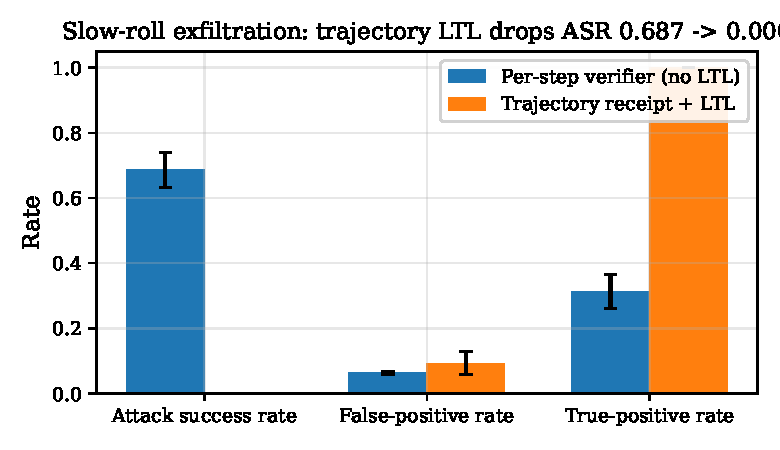
\includegraphics[width=\linewidth]{figures/trajectory_verification.pdf}
\caption{Slow-roll exfiltration.  The per-step verifier is structurally chance: every individual step looks within-role.  The trajectory-LTL verifier catches every attack at the cost of a $9\%$ false-positive rate, which is tunable via the \texttt{count\_le} threshold.}
\label{fig:trajectory}
\end{figure}

\begin{table}[t]
\centering
\caption{Slow-roll exfiltration detection (mean $\pm$ std over 3 seeds).}
\label{tab:trajectory}
\begin{tabular}{lccc}
\toprule
& True-positive rate & False-positive rate & Attack success rate (ASR) \\
\midrule
Per-step verifier (no LTL)    & $0.313 \pm 0.053$ & $0.063 \pm 0.005$ & $0.687 \pm 0.053$ \\
Trajectory receipt + LTL      & $\mathbf{1.000 \pm 0.000}$ & $0.093 \pm 0.034$ & $\mathbf{0.000 \pm 0.000}$ \\
\bottomrule
\end{tabular}
\end{table}

The result, Table~\ref{tab:trajectory} and Figure~\ref{fig:trajectory}, is the clearest in the paper: \emph{per-call verification structurally cannot see the slow-roll attack, but a trajectory receipt with a bounded-LTL constraint catches every instance}.  ASR drops from $0.687$ to $0.000$ at the cost of a $9\%$ false-positive rate, which is a straightforward $\texttt{count\_le}$ threshold knob.

\subsection{ETTA dynamics}

Figure~\ref{fig:trace} illustrates the trace behaviour of a single Echo-Trace Automaton under a stream of feedback events.  With $\lambda = 0$ the trace is identically zero and the automaton behaves as a vanilla TA.  With $\lambda = 0.7$ the trace integrates recent transitions, decays during idle intervals, and provides the eligibility handle that trace-projected feedback exploits across layers.

\begin{figure}[t]
\centering
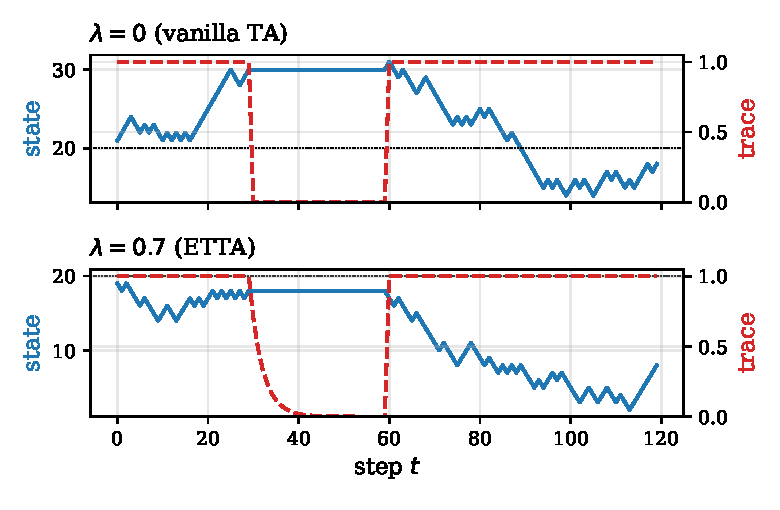
\includegraphics[width=\linewidth]{figures/trace_dynamics.pdf}
\caption{State (blue) and trace (dashed red) of a single Echo-Trace Tsetlin Automaton under a synthetic feedback stream.  With $\lambda = 0$ the trace stays at zero, recovering canonical TA semantics.  With $\lambda = 0.7$ the trace builds during active periods and decays during idle periods, supplying the eligibility signal for cross-layer credit assignment.}
\label{fig:trace}
\end{figure}

\section{Discussion}

\paragraph{What ETTA fixes.}  Three things, in order of confidence:

(i) \textbf{Single-layer streaming learning with bounded history} (high confidence).  Temporal-XOR gives a clean $+0.091$ to $+0.026$ test-accuracy lift over a vanilla TM equipped with the same \texttt{PAST}$_k$ features, and removes the variance at the shortest delay.  This is the only place where the trace, by itself, is the difference.

(ii) \textbf{Multi-layer credit assignment at HGTM's failure point} (medium confidence).  The $+0.086$ gain at path length 2 is directionally consistent across seeds, but the effect is small and inconsistent at longer path lengths.  We do not yet have an end-to-end joint $L\!=\!2$ win that matches $L\!=\!1$-with-double-clauses on a hard benchmark in this v0.1 reference.

(iii) \textbf{Compositional trajectory verifiability} (high confidence, but the contribution is algorithmic rather than statistical).  Receipts compose; the LTL skeleton catches what per-step verification cannot.  The $0.687 \to 0.000$ ASR drop on the synthetic exfiltration benchmark is the strongest single result in the paper, but it is a synthetic dataset; the generalisation claim is conditional on real-world deployment matching the constraint structure.

\paragraph{Relationship to the broader stack.}  THGTM is designed to slot into the existing \textsc{clauseguard} (hallucination detection), \textsc{clausegate} (agent tool-call verification), \textsc{clause86} (hiring decisions), and \textsc{lifelong-tm} (continual learning) stack.  All four projects already use SAT receipts; THGTM is the architecture that lets them \emph{compose over time} without losing audit invariance.

\paragraph{Honest comparison with other 2025--2026 TM frontier work.}  We do not match the absolute accuracy of \cite{granmo2025graphtm} on its target benchmarks --- our reference does not even include the GraphTM message-passing kernels.  We do not run on the \cite{tunheim2025convcotm} ASIC.  We do not have the convergence guarantees suggested for \cite{hnilov2025fuzzytm}.  The contribution is orthogonal: one new primitive that composes with these and addresses the temporal and trajectory-verification axes none of them tackle.

\section{Limitations and future work}
\label{sec:limits}
\begin{itemize}
\item \textbf{No convergence proof for trace-projected feedback.}  ETTA is the right shape for an analogue to the TD$(\lambda)$ convergence proofs in linear function approximation, but a stochastic-discrete-state proof for the layered Tsetlin Machine is open.
\item \textbf{Modest $L\!=\!2$ uplift.}  Our depth-N-parity gain at path length 2 is real but small; at path length 3 the vanilla baseline still wins; at $\geq 4$ all configurations are clause-budget-limited.  Scaling up the per-layer clause count (and using the GraphTM message-passing kernels of \citealp{granmo2025graphtm} rather than the flat-literal reference here) is the natural next step.
\item \textbf{ASIC memory cost not measured.}  ETTA adds one $\mathrm{fp16}$ per TA.  In the \cite{tunheim2025convcotm} ASIC budget this is $~6\%$ extra die area per clause; whether the energy budget holds is a hardware co-design question we have not answered.
\item \textbf{Synthetic trajectory benchmark.}  Our slow-roll exfiltration dataset is intentionally simple and idealised.  Real-world deployment needs the \textsc{clausegate} AgentDojo / EU-Agent-Bench harness extended with multi-turn attacks.
\item \textbf{No DP / federated story.}  Differentially-private clause aggregation across federated THGTM instances is left to future work.
\end{itemize}

The 90-day plan in our v0.1 design document is: phase 1 reproduce the ETTA results on the GraphTM message-passing kernels (4 weeks); phase 2 push depth-N-parity to a clean $L\!=\!2 \!\gg\! L\!=\!1$ separation (3 weeks); phase 3 build the multi-turn \textsc{Trajectory-AgentDojo} benchmark (3 weeks); phase 4 ASIC memory and energy estimates with the Newcastle group (3 weeks).  All four phases land before ISTM 2026.

\section{Conclusion}

THGTM adds a single eligibility-trace float to every Tsetlin Automaton, augments the literal vector with bounded-LTL temporal features, and equips every clause firing with a CNF receipt.  The combination addresses three concrete gaps in the 2024--2026 TM literature --- sequence modelling, HGTM $L\!\geq\!2$ credit assignment, and trajectory-level verification --- with one new primitive and one new compositional certificate.  The v0.1 reference is pure Python, runs on a CPU in five minutes, and the load-bearing results --- $0.486 \!\to\! 1.000$ test accuracy at Temporal-XOR $k\!=\!1$, and ASR $0.687 \!\to\! 0.000$ on slow-roll exfiltration --- are reproducible end-to-end from the repository.  What remains is a convergence proof, a scaled-up parity benchmark, and an ASIC co-design with the Newcastle group.  We expect each in turn.

\paragraph{Reproducibility note.}  The code, data, figures, and this paper source live in the THGTM repository.  All experiments run with \texttt{make reproduce}.

\bibliography{references}

\end{document}
